\documentclass[]{article}

%opening
\title{4F13 Probabilistic Machine Learning - True Skill Ranking}
\author{Lawrence Tray \\ St John's College}

%packages
\usepackage[margin=0.5in]{geometry}
\usepackage[export]{adjustbox}
\usepackage{graphicx}
\usepackage{amsmath}
\usepackage{amssymb}
\usepackage{hyperref}
\usepackage{caption}
\usepackage{subcaption}
\usepackage{parskip}
\usepackage{listings}
\usepackage{pdfpages}

%package setup
\graphicspath{{./img/}}
\DeclareMathOperator*{\argmax}{arg\,max}
\DeclareMathOperator*{\argmin}{arg\,min}

%custom commands
\newcommand{\dft}{\mathcal{F}}
\newcommand{\idft}{\mathcal{F}^{-1}}
\newcommand{\Xcal}{\mathcal{X}}
\newcommand{\Ncal}{\mathcal{N}}
\newcommand{\cmplx}{\mathbb{C}}
\newcommand{\Lcal}{\mathcal{L}}
\newcommand{\figwidth}{0.6\linewidth}

%section numbering
\renewcommand{\thesubsection}{\thesection.\alph{subsection}}

\begin{document}

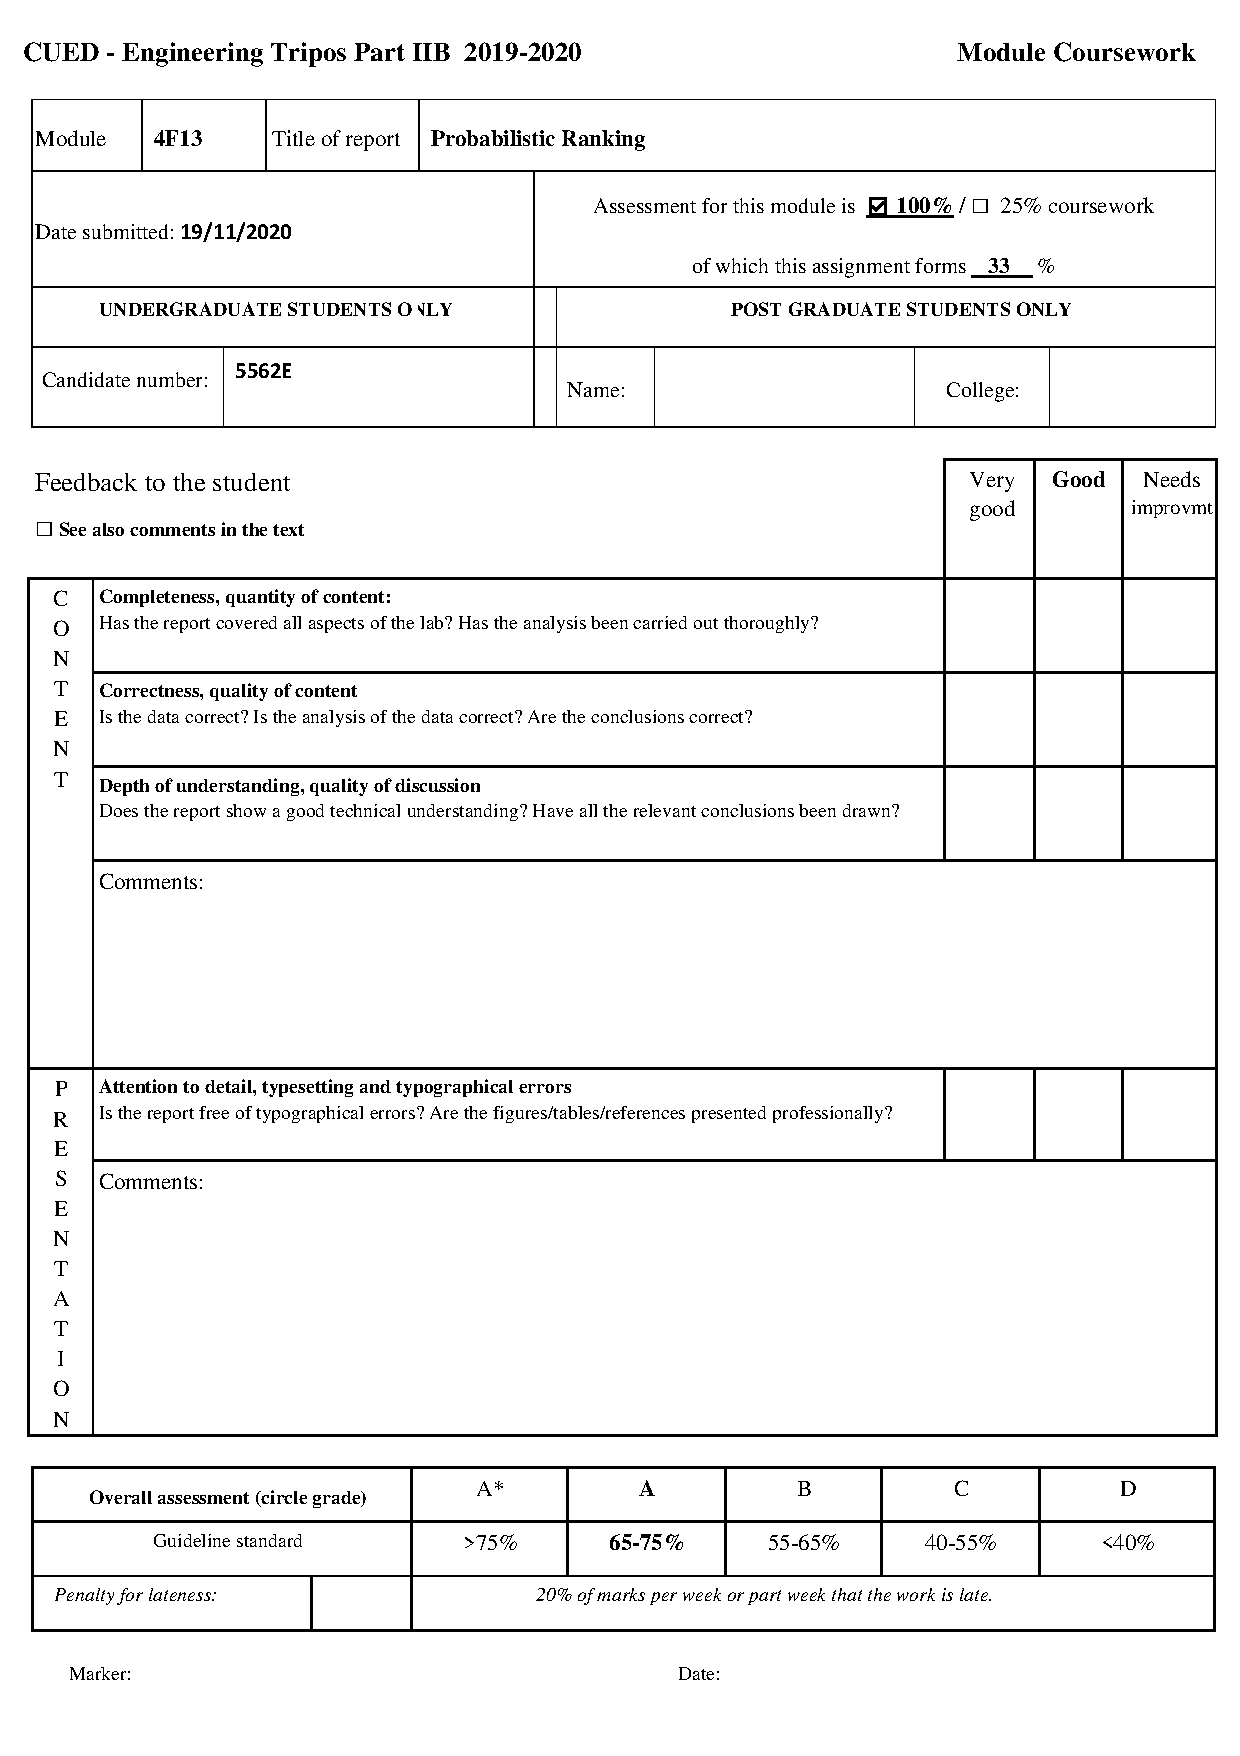
\includepdf[pages={1}]{coversheet-CW2.pdf}

\setcounter{page}{1}
\maketitle

\begin{abstract}
This report outlines the results of the second coursework for 4F13. 
\end{abstract}

\tableofcontents

\section{Questions}
\subsection{Gibbs Sampling}

\begin{lstlisting}[frame=single, caption={Gibbs sampling additions}, label={lst:gibbs}, language={python}]
m = np.zeros((M, 1))
for p in range(M):
	# fill in m[p] prediction (natural param conditional)
	wins_array = np.array(G[:, 0] == p).astype(int)
	loss_array = np.array(G[:, 1] == p).astype(int)
	m[p] = np.dot(t[:,0], (wins_array - loss_array))
	
iS = np.zeros((M, M))  # Container for sum of precision matrices (likelihood terms)
for g in range(N):
	# Build the iS matrix
	winner = G[g, 0]
	loser = G[g, 1]
	
	iS[winner, winner] += 1
	iS[winner, loser] -= 1
	iS[loser, winner] -= 1
	iS[loser, loser] += 1
\end{lstlisting}

\subsection{EP - Message Passing}


\subsection{EP - Top Four Head to Head}

\begin{table}[!h]
	\subfloat[Prob. row player is more skilful]{
		\begin{tabular}{c | c c c c}
			$P(w_i > w_j)$ & \textbf{Djokovic} & \textbf{Federer} & \textbf{Nadal} & \textbf{Murray} \\ \hline
			\textbf{Djokovic}      & -                 & 0.92             & 0.95           & 0.98            \\
			\textbf{Federer}       & 0.08              & -                & 0.59           & 0.79            \\
			\textbf{Nadal}         & 0.05              & 0.41             & -              & 0.73            \\
			\textbf{Murray}        & 0.02              & 0.21             & 0.27           & -              
		\end{tabular}
	}
	\subfloat[Prob. row player wins a head-to-head]{
		\begin{tabular}{c | c c c c}
			$P(t_{ij} > 0)$ & \textbf{Djokovic} & \textbf{Federer} & \textbf{Nadal} & \textbf{Murray} \\ \hline
			\textbf{Djokovic}      & -                 & 0.64             & 0.66           & 0.71            \\
			\textbf{Federer}       & 0.36              & -                & 0.52           & 0.58            \\
			\textbf{Nadal}         & 0.34              & 0.48             & -              & 0.56            \\
			\textbf{Murray}        & 0.29              & 0.42             & 0.44           & -              
		\end{tabular}
	}
	\caption{Top four players comparison}
	\label{tab:top-4}
\end{table}


\subsection{Gibbs - Nadal v Djokovic}


\subsection{Method Comparison: Win ratio, Gibbs and EP}

\textbf{Words}: 987

\end{document}
